\documentclass[tikz,border=5pt]{standalone}
\usepackage{pgfplots}
\usepackage{amsmath}
\pgfplotsset{compat=1.18}
\usepgfplotslibrary{fillbetween}
\usepgfplotslibrary{groupplots}

\definecolor{corba}{HTML}{3F51B5}
\definecolor{segona}{HTML}{2E9D5B}
\definecolor{tercera}{HTML}{D97706}
\definecolor{maxim}{HTML}{D32F2F}
\definecolor{extrem}{HTML}{374151}
\definecolor{estalvi}{HTML}{E3E8F7}

\begin{document}
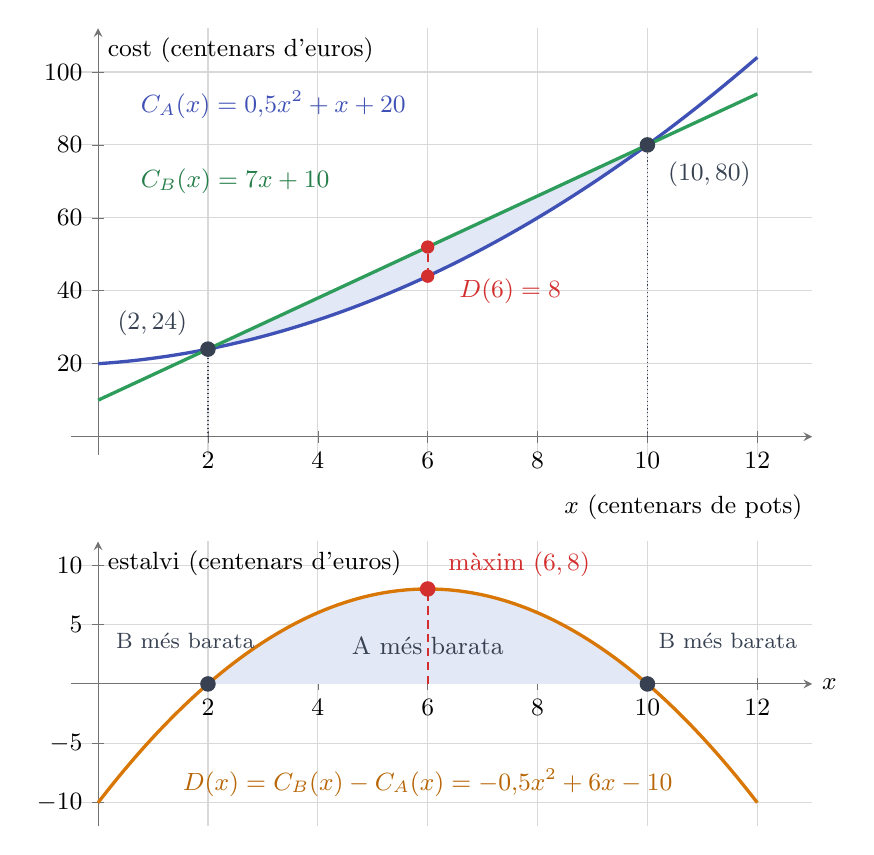
\begin{tikzpicture}
  \begin{groupplot}[
    group style={group size=1 by 2, vertical sep=1.1cm},
    width=11cm,
    axis lines=middle,
    xmin=-0.5,
    xmax=13,
    xtick={0,2,4,6,8,10,12},
    grid=major,
    grid style={black!15},
    axis line style={black!55},
    tick style={black!55},
    tick label style={font=\small},
    label style={font=\small},
    clip=false,
  ]
    % ------------------------------------------------ costos de les dues màquines
    \nextgroupplot[
      height=7cm,
      ymin=-5,
      ymax=112,
      ytick={0,20,40,60,80,100},
      xlabel={$x$ (centenars de pots)},
      xlabel style={at={(axis description cs:1,-0.07)}, anchor=north east},
      ylabel={cost (centenars d'euros)},
    ]
      \addplot[draw=none, domain=2:10, samples=80, name path=A]
        {0.5*x^2+x+20};
      \addplot[draw=none, domain=2:10, samples=2, name path=B]
        {7*x+10};
      \addplot[fill=estalvi, draw=none] fill between[of=A and B];

      \addplot[corba, very thick, domain=0:12, samples=160]
        {0.5*x^2+x+20};
      \addplot[segona, very thick, domain=0:12, samples=2]
        {7*x+10};

      \draw[maxim, thick, densely dashed]
        (axis cs:6,44) -- (axis cs:6,52);
      \draw[extrem, densely dotted]
        (axis cs:2,0) -- (axis cs:2,24);
      \draw[extrem, densely dotted]
        (axis cs:10,0) -- (axis cs:10,80);

      \addplot[only marks, mark=*, mark size=2.6pt, extrem]
        coordinates {(2,24) (10,80)};
      \addplot[only marks, mark=*, mark size=2.2pt, maxim]
        coordinates {(6,44) (6,52)};

      \node[anchor=south east, text=extrem, font=\small]
        at (axis cs:1.8,25) {$(2,24)$};
      \node[anchor=north west, text=extrem, font=\small]
        at (axis cs:10.2,78) {$(10,80)$};
      \node[anchor=west, text=maxim, font=\small]
        at (axis cs:6.4,40) {$D(6)=8$};

      \node[anchor=west, text=corba, font=\small]
        at (axis cs:0.6,91) {$C_A(x)=0{,}5x^2+x+20$};
      \node[anchor=west, text=segona!80!black, font=\small]
        at (axis cs:0.6,70) {$C_B(x)=7x+10$};

    % ------------------------------------------------ funció diferència
    \nextgroupplot[
      height=5.2cm,
      ymin=-12,
      ymax=12,
      ytick={-10,-5,0,5,10},
      xlabel={$x$},
      xlabel style={at={(axis cs:13,0)}, anchor=west},
      ylabel={estalvi (centenars d'euros)},
    ]
      \addplot[draw=none, domain=2:10, samples=80, name path=D]
        {-0.5*x^2+6*x-10};
      \addplot[draw=none, domain=2:10, samples=2, name path=Z]
        {0};
      \addplot[fill=estalvi, draw=none] fill between[of=D and Z];

      \addplot[tercera, very thick, domain=0:12, samples=160]
        {-0.5*x^2+6*x-10};

      \draw[maxim, thick, densely dashed]
        (axis cs:6,0) -- (axis cs:6,8);

      \addplot[only marks, mark=*, mark size=2.6pt, extrem]
        coordinates {(2,0) (10,0)};
      \addplot[only marks, mark=*, mark size=2.6pt, maxim]
        coordinates {(6,8)};

      \node[anchor=south west, text=maxim, font=\small]
        at (axis cs:6.2,8.2) {màxim $(6,8)$};

      \node[anchor=center, text=tercera!85!black, font=\small]
        at (axis cs:6,-8.3) {$D(x)=C_B(x)-C_A(x)=-0{,}5x^2+6x-10$};
      \node[anchor=center, text=extrem, font=\small]
        at (axis cs:6,3.2) {A més barata};
      \node[anchor=west, text=extrem, font=\footnotesize]
        at (axis cs:0.15,3.6) {B més barata};
      \node[anchor=east, text=extrem, font=\footnotesize]
        at (axis cs:12.9,3.6) {B més barata};
  \end{groupplot}
\end{tikzpicture}
\end{document}
